\subsection{Utledning av bølgeligningen}
\subsubsection{Forhåndsbetingelser}
For å finne frem til bølgeligningen må en se på hvordan systemet en skal bruke likningen i ser ut.
På en gitar er lengden på strengen justerbar, men en endrer tonen ved å stramme eller slakke
på gitarstrengen.

En gitarstreng kan modelleres som en tråd som er spent mellom to punkter, der den er fiksert på plass.
I normaltilstand ligger strengen spent i en rett linje mellom punktene, frem til den blir plukket. Da
har den blitt forstyrret, og strengen begynner å vibrere. Problemet er da å finne en \(u(x,t)\) som modellerer
defleksjonen til strengen. Hvis strengen har lengde \(l\), massetetthet \(\rho\) og blir sluppet løs ved \(t=0\),
vil formelen finne defleksjonen til strengen for hvilken som helst \(x\) når \(t>0\).

For å løse likningen trengs det noen forhåndsbetingelser.

\begin{enumerate}
  \item Gravitasjon er neglisjerbar i forhold til strengspenningen.
  \item Alle defleksjoner er små og skjer i samme plan.
  \item Massen per lengde er konstant over hele strengen, slik at spenningen er den samme
  gjennom hele strengen.
\end{enumerate}

\subsubsection{Utledning}

\begin{figure}[h]
\centering
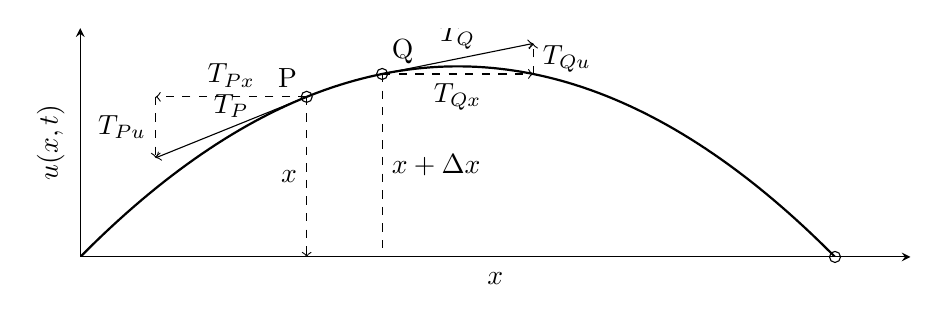
\begin{tikzpicture}
\begin{axis}[
  width=\textwidth,
  height=0.37\textwidth,
  axis lines=left,
  xlabel={$x$},
  ylabel={$u(x,t)$},
  xmin=0, xmax=1.1,
  ymin=0, ymax=0.6,
  xtick=\empty,
  ytick=\empty
]
  % punkter
  \coordinate (Ppoint)  at (axis cs:0.3,0.42);
  \coordinate (Pupoint) at (axis cs:0.1,0.26);
  \coordinate (Pxpoint) at (axis cs:0.1,0.42);
  \coordinate (Qpoint)  at (axis cs:0.4,0.48);
  \coordinate (Qupoint) at (axis cs:0.6,0.56);
  \coordinate (Qxpoint) at (axis cs:0.6,0.48);

  % strengkurve
  \addplot[domain=0:1, samples=100, thick] {-2*x^2 + 2*x};

  % krefter ved P
  \draw[->, thin] (Ppoint) -- (Pupoint) node[midway, above] {$T_P$};
  \draw[->, thin, dashed] (Ppoint) -- (Pxpoint) node[midway, above] {$T_{Px}$};
  \draw[->, thin, dashed] (Pxpoint) -- (Pupoint) node[midway, left]  {$T_{Pu}$};

  % krefter ved Q
  \draw[->, thin] (Qpoint) -- (Qupoint) node[midway, above] {$T_Q$};
  \draw[->, thin, dashed] (Qpoint) -- (Qxpoint) node[midway, below] {$T_{Qx}$};
  \draw[->, thin, dashed] (Qxpoint) -- (Qupoint) node[midway, right] {$T_{Qu}$};

  % loddrette hjelpelinjer
  \draw[->, dashed] (axis cs:0.3,0.42) -- (axis cs:0.3,0) node[midway, left] {$x$};
  \draw[dashed]     (axis cs:0.4,0.48) -- (axis cs:0.4,0) node[midway, right] {$x+\Delta x$};

  % punktsymboler og etiketter
  \addplot[only marks, mark=o] coordinates {(0.3,0.42) (0.4,0.48) (1,0)};
  \node[anchor=south east] at (Ppoint) {P};
  \node[anchor=south west] at (Qpoint) {Q};
  \node[anchor=north]      at (axis cs:1,0) {$l$};

  % ! Fjernet vinkler her for å unngå feilmeldinger.

\end{axis}
\end{tikzpicture}
\caption{Krefter og vinkler på et lite strengstykke \([x,\,x+\Delta x]\).}
\end{figure}

For å finne likningen tar vi for oss en liten bit av strengen ved \(t=0\), som er \(\Delta x\) lang og starter på
\(x\). Vi setter punkt \(P=(x,u(x,0))\) og punkt \(Q=(x+\Delta x, u(x+\Delta x,0))\).
\(T\) er kraften spenningen i strengen skaper på ett punkt \(x>0\) langs strengen. Vi definerer
\(\alpha\) til å være vinkelen mellom \(T_{Qx}\) og \(T_Q\), og \(\beta\) til å være vinkelen mellom
\(T_{Px}\) og \(T_P\).

\begin{align*}
  T_{Px} = T_P \cos\beta, &\qquad T_{Qx} = T_Q \cos\alpha,\\
  T_{Pu} = T_P \sin\beta, &\qquad T_{Qu} = T_Q \sin\alpha.
\end{align*}

Fordi vi satte at spenningen i strengen er lik over hele strengen, vil de horisontale kreftene
av \(T_Q\) og \(T_P\) utjevne hverandre:

\begin{equation}
  T_{Px} = T_{Qx} = T = \text{const.}
  \label{eq:horisontaleKrefterKonstant}
\end{equation}

Ser vi på Newtons andre lov \((F=ma)\) for strengstykket, kan vi sette massen \(m=\rho\,\Delta x\) og
akselerasjonen \(a=u_{tt}\). Kraften som blir påført strengen er \(F=T_{Qu}-T_{Pu}\). Da får vi

\begin{equation*}
  T_{Qu}-T_{Pu}=\rho\,\Delta x\,\frac{\partial^2 u}{\partial t^2}.
\end{equation*}

Bruker vi \(\tan\theta=\frac{\sin\theta}{\cos\theta}\) og \eqref{eq:horisontaleKrefterKonstant}, samtidig
som vi vet at \(\tan\alpha\) og \(\tan\beta\) beskriver stigningstallet til tangenten i henholdsvis \(Q\) og \(P\), får vi

\begin{equation}
  \frac{T_{Qu}}{T_{Qx}}-\frac{T_{Pu}}{T_{Px}}
  = \tan\alpha - \tan\beta
  = \frac{\partial u}{\partial x}(x+\Delta x,t)-\frac{\partial u}{\partial x}(x,t)
  = \frac{\rho\,\Delta x}{T}\,\frac{\partial^2 u}{\partial t^2}.
  \label{eq:krefterPaStykke}
\end{equation}

Ganger vi begge sider med \(\dfrac{T}{\rho\,\Delta x}\) får vi

\begin{equation}
  \frac{\partial^2 u}{\partial t^2}
  = \frac{T}{\rho\,\Delta x}\left[
     \frac{\partial u}{\partial x}(x+\Delta x,t)-\frac{\partial u}{\partial x}(x,t)
    \right].
  \label{eq:tidPartiellDerivert}
\end{equation}

Lar vi \(\Delta x\to 0\), kjenner vi igjen definisjonen av den deriverte:

\begin{equation}
  \frac{\partial^2 u}{\partial t^2}
  = \lim_{\Delta x\to 0}\frac{T}{\rho}\frac{1}{\Delta x}
    \left[\frac{\partial u}{\partial x}(x+\Delta x,t)-\frac{\partial u}{\partial x}(x,t)\right]
  = \frac{T}{\rho}\,\frac{\partial^2 u}{\partial x^2}.
  \label{eq:deltaXGarMotNull}
\end{equation}

Setter vi \(c^2=\dfrac{T}{\rho}\) får vi bølgeligningen

\begin{equation}
  \frac{\partial^2 u}{\partial t^2}
  = c^2\,\frac{\partial^2 u}{\partial x^2},
  \qquad
  c^2=\frac{T}{\rho}.
  \label{eq:utledetBolgelikning}
\end{equation}

\subsection{Valg av løsningmetode for numerisk løsning}
\subsubsection{Valg av verktøy}
For å løse bølgelikningen numerisk, har vi valgt å bruke Python. Dette er et programmeringsspråk som er mye brukt innenfor vitenskapelige
beregninger, og har et stort utvalg av biblioteker som gjør det enkelt å implementere numeriske metoder og visualisere resultater. Innenfor 
bibliotekene numpy og matplotlib, finnes det mange funksjoner som gjør det enkelt å løse oppgaver numerisk og plotte visuelle fremstillinger.
Dette gjør Python til et godt valg for å løse bølgelikningen numerisk. For å lage animasjoner av resultatene, har vi valgt å bruke biblioteket 
matplotlib.animation, som er en del av matplotlib-biblioteket. Dette lar brukeren få en bedre forståelse av hvordan løsningen utvikler seg over tid.
For å plotte grafen har vi brukt matplotlib.pyplot, som er et vanlig grafikkbibliotek i Python. Dette biblioteket gjør det enkelt å lage 2D-grafer og 
visualisere data. For å forstå komplekse lignigner som bølgeligningen er essensielt å kunne visualisere resultatene på en enkel måte.

\subsubsection{Løsning med separasjon av variable}
\dots

\begin{equation}
	u_{tt} = c^2 u_{xx} \qquad \iff \qquad 
	\frac{\partial^2 u}{\partial t^2} = \frac{T}{\rho} \frac{\partial^2 u}{\partial x^2}	
	\label{eq:bølgelikningForLøsning}
\end{equation}

For å løse bølgelikningen, trenger vi noen grense- og initial-betingelser. Vi vet at strengen har en fast lengde $l$,
og er festet i begge ender, dette er grensebetingelsene. Initialbetingelsene skjer ved $t=0$, og da blir strengen
sluppet løs av en kraft, som har påvirket strengen til å slippes fra en posisjon bestemt av $f(x)$.

\subsubsection{Grensebetingelser}

\begin{align}
	u(0 , t) = 0 \label{eq:grensebetingelse0}\\
	u(l , t) = 0 \label{eq:grensebetingelsel}
\end{align}

\subsubsection{Initialbetingelser}

\begin{equation}
	u(x , o) = f(x) = \sum_{n=0}^{n=\infty} c_n \sin \left( \frac{n \pi}{l} x \right) 	
	\label{eq:initialbetingelse}
\end{equation}

(\ref{eq:initialbetingelse}) tilsier at ved $t=0$ er 




\subsection{Beskrivelse av kode for numerisk løsning}
\subsubsection{Pakker, variabler og parametere}
Først importeres nødvendige pakker for å kunne utføre numeriske beregninger og plotte grafiske fremstillinger. Her
tar vi i bruk numpy for numeriske operasjoner, matplotlib.pyplot for plotting, og matplotlib.animation for å lage 
animasjoner slik som forklart i forrige seksjon. Deretter setter vi konfigurajsonsparametere som definerer
fysiske egenskaper til strengen, samt parametere for den numeriske løsningen. Dette inkluderer lengden $L$ på strengen,
bølgehastigheten $c$ og tiden $s$ vi ønsker å simulere. Videre defineres antall punkter $N$ som skal brukes til å dele 
opp strengen. Dette påvirker nøyaktigheten til den numeriske løsningen, der flere punkter gir en mer nøyaktig løsning,
men øker beregningstid og ressursbruk. Videre definerer vi modi for funksjonen, som er antall bølgetopper som skal være 
tilstede for å lage startformen, hvor en høyere verdi gir skarpere kanter og høyere detaljnivå. \parencite{bølgeSimulering} 
For å fremvise en fysisk simulering av en gradvis tykkere streng, kan vi i stedet for å øke $\rho$, senke bølgefarten $c$ i 
henhold til (\ref{eq:bølgefart}).

Videre setter vi opp betingelser for den grafiske fremstillingen, slik som FPS (frames per second) for animasjonen, og
tykkelsen for linjen på grafen. For å sette startformen på grafen setter vi 

\begin{verbatim}
  initial_shape_type = "pluck"
  pluck_width: float = 0.15
\end{verbatim}

hvor \verb|"pluck"| indikerer at grafen (i dette tilfellet en streng) skal strekkes, og \verb|pluck_width| definerer hvor bredt området som strekkes er.

\subsubsection{Initialbetingelser funksjonen}


\subsubsection{}
\dots
